%\newcommand{\eps}{\epsilon}
\newcommand{\Pmax}{p_\text{max}} 	
\newcommand{\Hint}{H_{int}}
\newcommand{\kbar}{\bar{k}}
\newcommand{\Delk}{\Delta}
\newcommand{\Sumk}{\Sigma}
\newcommand{\Qrot}{Q_{pq}(\tau_s)}
\newcommand{\shapecor}{\mathcal{S}}
\newcommand{\ampcor}{\mathcal{A}}
\newcommand{\totalcor}{\mathcal{E}}
\newcommand{\threeLs}{L_p(\kbar_1)L_q(\kbar_2)L_r(\kbar_3)}
\newcommand{\threePs}{P_p(\kbar_1)P_q(\kbar_2)P_r(\kbar_3)}
\newcommand{\threeQs}{Q_p(k_1)Q_q(k_2)Q_r(k_3)}
\newcommand{\Lbasic}{\mathcal{P}_0}
\newcommand{\Linvk}{\mathcal{P}_1}
\newcommand{\Lnsinv}{\mathcal{P}^{n_s}_1}
\newcommand{\Lnsboth}{\mathcal{P}^{n_s}_{01}}
\newcommand{\Linvksq}{\mathcal{P}_2}
\newcommand{\Lns}{\mathcal{P}^{n_s}_2}
\newcommand{\Fbasic}{\mathcal{F}_0}
\newcommand{\Finvk}{\mathcal{F}_1}
\newcommand{\Finvksq}{\mathcal{F}_2}
\newcommand{\quadpot}{V_{\phi^2}(\phi)}
%\newcommand{\threeqs}{q_p(\kbar_1)\,q_r(\kbar_2)\,q_s(\kbar_3)}
\newcommand{\threeqs}{q_p(k_1)\,q_r(k_2)\,q_s(k_3)}
\newcommand{\threeqstilde}{q_{\tilde{p}}(k_1)\,q_{\tilde{r}}(k_2)\,q_{\tilde{s}}(k_3)}
\newcommand{\kmin}{{k_\text{min}}}
\newcommand{\kmax}{{k_\text{max}}}
\newcommand{\fnl}{f_{NL}}
\newcommand{\fnllocal}{f^{local}_{NL}}
\newcommand{\fnlequil}{f^{equil}_{NL}}
\newcommand{\fnlortho}{f^{ortho}_{NL}}

\chapter{An Inflationary Constraint from the $\cmb$ Bispectrum}\label{chapter:constraints}
\section{DBI sound speed constraint}
    The result we get is different, but not surprisingly different.
    The possible reasons for this are the fact we are using slightly different
    scales (since we are limited to $\kmax/\kmin=1000$ for convergence reasons we cannot
    use all the scales in the $\planck$ data), convergence in the number of maps
    ($\modal$ uses $\tilde300$ while $\cmbbest$ uses $140$) or possibly numerical issues,
    implementation error. See~\cite{Sohn_2021} for an in-depth discussion of these possibilities
    \textcolor{red}{summarise here}.
    \begin{figure}[htbp!]
        \centering
        %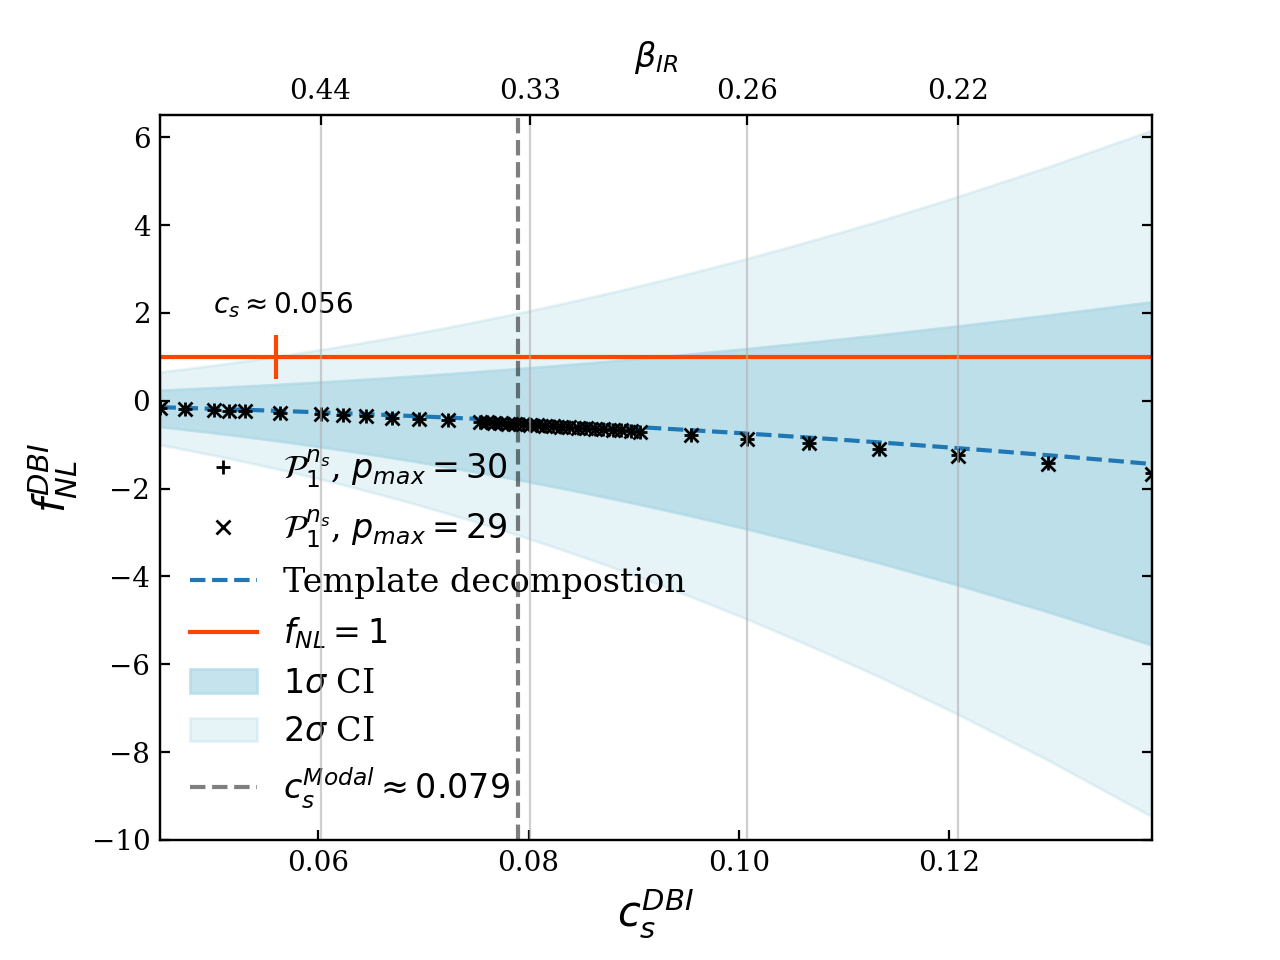
\includegraphics[width=0.9\textwidth]{wuhyun_plots/beta_ir_constraint_busy.png}
        \includegraphics[width=0.9\textwidth]{wuhyun_plots/beta_ir_constraint_with_beta.png}
        \caption{
            Our constraint on DBI inflation. Here $c_s^{DBI}$ is not an input parameter
            (unlike in the template case), instead it is time dependent, and the plotted
            value is taken from the horizon crossing of the pivot scale. We find that $\beta_{IR}<0.5$
            %0.464
            is outside of our $2\sigma$ confidence interval. This plot was obtained by
            scanning across values of $\beta_{IR}$ and calculating the corresponding primordial bispectra
            using $\primodal$, then projecting those bispectra onto the $\cmb$
            and comparing them to the $\planck$ $\cmb$ temperature data using
            $\cmbbest$. Since the amplitude is fixed by the scenario, we rule out a
            scenario by ruling out $f_{NL}^{DBI}=1$.
            We can see that the $\cmbbest$ result does not agree with the $\modal$ result,
            but as we see in figure~\ref{fig:equil_constraints_comparison},
            the discrepancy is not unexpected. We discuss possible explanations
            in the text.
            Note that the $\beta_{IR}$ is approximately proportional to $\left(c^*_s\right)^{-2}$.
        }\label{fig:dbi_sound_speed_scan_beta}
    \end{figure}

    In this chapter, we 
    use $\planck$ data to place a constraint on the sound speed in DBI inflation.
    We then compare this result to the same constraint obtained in the $\planck$
    analysis~\cite{Planck_NG_2018},
    with the aim of validating the full $\primodal$-$\cmbbest$ pipeline.
    The $\planck$ result was obtained by constraining the amplitude
    of the DBI template, and using a slow-roll relation to map this
    to a constraint on the sound speed.
    In our pipeline, however, we scan over a fundamental parameter of the model,
    and the sound speed (more precisely $c_s^*$, the sound speed at horizon crossing of
    the pivot scale) is a calculated quantity.
    We obtain the full shape and amplitude information (within our $k$-range) for
    each scenario in our scan and the final
    constraint makes use of the entirety of that information, up to
    convergence in $\Pmax$.


    Equation (55) in~\cite{Planck_NG_2018} presents the 
    constraint on the sound speed during DBI inflation
    derived from the $\cmb$ bispectrum
    \begin{align}\label{eq:planck_dbi_constraint}
        c_s^{DBI}&\ge0.079\qquad(95\%,~T~\text{only})
    \end{align}
    using the definition~\eqref{fnl_dbi_defn}.
    While our goal is to validate our pipeline by reproducing this constraint,
    we would not expect to reproduce it exactly.
    This is due to numerous effects, including
    \textcolor{red}{Lack of maps? Different approximations? Numerics?},
    as discussed in detail in~\cite{Sohn_2021}.
    We can however understand the expected variance of such estimators by simply examining the
    scatter between the estimators used in the $\planck$ analysis.
    We show this in figure~\ref{fig:equil_constraints_comparison} for the equilateral template~\eqref{equil_shape}
    which is closely related to the DBI template.


    \begin{figure}[htbp!]
        \centering
        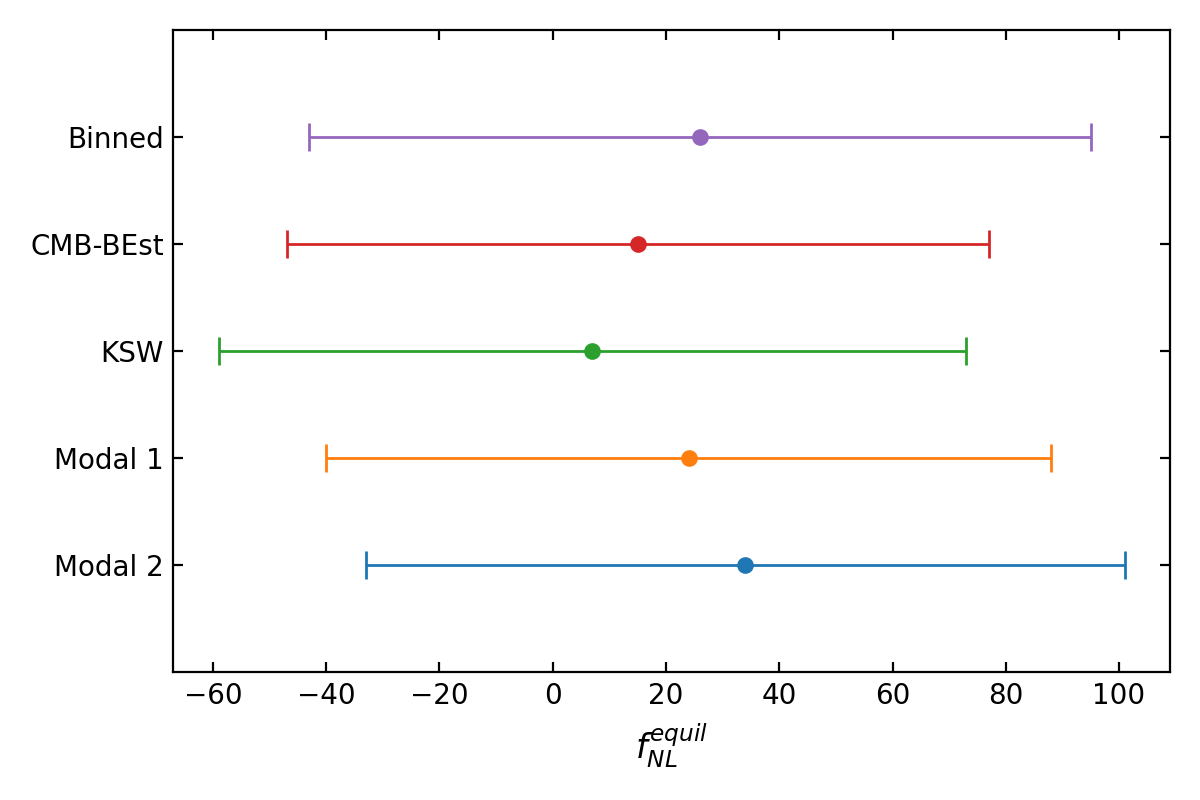
\includegraphics[width=0.9\textwidth]{wuhyun_plots/fnl_equil_planck_scatter.png}
        \caption{
            A comparison of the various estimation methods used in $\planck$,
            as presented in table 5 of~\cite{Planck_NG_2018},
            with the $\cmbbest$ result, presented in~\cite{Sohn_2021}.
            We plot the constraints obtained by each method for $\fnlequil$,
            along with their $68\%$ uncertainty margin.
            Note that all the estimation methods use the same data
            \textcolor{red}{and maps},
            and are near optimal, hence their uncertainty margins are close
            to identical.
            We see that while the estimators do not agree, there is no discrepancy with any
            significance---in particular, we see that $\cmbbest$ is not an outlier.
            Possible contributions to the difference in the central values are convergence in each
            method (for their respective convergence parameters), implementation error,
            and numerical stability.
            The $\cmbbest$ result quoted here was obtained by decomposing the equilateral
            template~\eqref{equil_shape} (using definition~\eqref{planck_fnl_defn_ns} for $\fnlequil$)
            in the $\Lnsinv$ basis for $\Pmax=30$.
            \textcolor{red}{Which is the abstract one in Planck?}
        }\label{fig:equil_constraints_comparison}
    \end{figure}


\section{Connecting to $\cmbbest$}
The potential we use is the IR one discussed in~\cite{Bean_ir_dbi} as discussed \textcolor{red}{earlier}.
See also~\cite{Chen_dbi, warp_features_dbi} for useful discussions. \textcolor{red}{Reasons.}

    We use equation~\eqref{eq:dbi_warp}, which has four free parameters,
    $\beta_{IR}$, $\lambda_{DBI}$, $\phi_0$, and $V_0$.
    We use $\beta_{IR}$ to parameterise our scan,
    $\beta_{IR}\in[0.1885, 0.58]$.
We hold $\lambda_{DBI}=2.00475\times10^{15}$, $V_0 = 5.2\times10^{-12}$
and $\phi_0 = 0.46042$ fixed.
We start the background evolution on the slow-roll attractor, finding initial conditions which
satisfy the Friedman constraint, as discussed in section~\ref{sec:interactions}.
    For each scenario in this scan we ensure that $\ln\left(10^{10}A_s\right)$
    is within $3.044\pm0.014$,
    and that $n_s^{*}$ is within $0.9649\pm0.0042$.


    We find that $\beta_{IR}=0.331$ produces $c_s^{*}=0.0794$,
    which is close to the $\planck$ constraint~\eqref{eq:planck_dbi_constraint}.
    Thus, we roughly expect to find that $\beta_{IR}<0.331$ is ruled out
    (for all the other scenario parameters held fixed at the above values).


%    \begin{tabular}{lrrrrrrrrrr}
%        \toprule
%        $\beta_{IR}$ &    $c_s^{*}$ &  $\varepsilon_s^{*}$ &   $\varepsilon^{*}$ &   $n_s^{*}$ &  $n_{NG}^{*}$ &   $\phi^{*}$ &     $H^{*}$ &   $\eta^{*}$ \\
%        \midrule
%        $1.89\times 10^{-1}$  &  $1.39\times 10^{-1}$  &  $  8.57\times 10^{-3}$  &  $7.44\times 10^{-5}$  &  $-3.50\times 10^{-2}$  &  $-8.72\times 10^{-2}$  &  $5.19\times 10^{-1}$  &  $1.31\times 10^{-6}$  &  $2.63\times 10^{-2}$ \\
%        $5.80\times 10^{-1}$  &  $4.50\times 10^{-2}$  &  $  8.67\times 10^{-3}$  &  $2.31\times 10^{-4}$  &  $-3.63\times 10^{-2}$  &  $-8.99\times 10^{-2}$  &  $5.15\times 10^{-1}$  &  $1.30\times 10^{-6}$  &  $2.71\times 10^{-2}$ \\
%        \bottomrule
%    \end{tabular}
    In table~\ref{tab:scan_summary_sr} we summarise the slow-roll parameters for the scan,
    in table~\ref{tab:scan_summary_bkgd} we summarise the background parameters,
    and in table~\ref{tab:scan_summary_ns} we summarise the resulting scaling indices.
    \\
    \\
\begin{table}[h!]
  \begin{center}
    \begin{tabular}{lrrrrrrr}
        \toprule
        $\beta_{IR}$ &    $c_s^{*}$ &  $\varepsilon_s^{*}$ &   $\varepsilon^{*}$ &   $\eta^{*}$ \\
        \midrule
        $1.89\times 10^{-1}$  &  $1.39\times 10^{-1}$  &  $  8.57\times 10^{-3}$  &  $7.44\times 10^{-5}$  &  $2.63\times 10^{-2}$ \\
        $5.80\times 10^{-1}$  &  $4.50\times 10^{-2}$  &  $  8.67\times 10^{-3}$  &  $2.31\times 10^{-4}$  &  $2.71\times 10^{-2}$ \\
        \bottomrule
    \end{tabular}
    \caption{Summary of slow-roll parameters across the scan.}\label{tab:scan_summary_sr}
  \end{center}
\end{table}
    \\
    \\
\begin{table}[h!]
  \begin{center}
    \begin{tabular}{lrrr}
        \toprule
        $\beta_{IR}$ &  $\phi^{*}$ &     $H^{*}$ \\
        \midrule
        $1.89\times 10^{-1}$  &  $5.19\times 10^{-1}$  &  $1.31\times 10^{-6}$\\
        $5.80\times 10^{-1}$  &  $5.15\times 10^{-1}$  &  $1.30\times 10^{-6}$\\
        \bottomrule
    \end{tabular}
    \caption{Summary of scenario parameters across the scan.}\label{tab:scan_summary_bkgd}
  \end{center}
\end{table}
    \\
    \\
\begin{table}[h!]
  \begin{center}
    \begin{tabular}{lrrrrrrr}
        \toprule
        $\beta_{IR}$ &  $n_s^{*}$ &  $n_{NG}^{*}$\\
        \midrule
        $1.89\times 10^{-1}$  &  $9.650\times 10^{-1}$  &  $-8.72\times 10^{-2}$\\
        $5.80\times 10^{-1}$  &  $9.637\times 10^{-1}$  &  $-8.99\times 10^{-2}$\\
        \bottomrule
    \end{tabular}
    \caption{Summary of scaling indices across the scan.}\label{tab:scan_summary_ns}
  \end{center}
\end{table}


\begin{figure}[!pth]
\centering
\includegraphics[width=\columnwidth]{dbi_scan_template_corrs_plots/dbi_primodal_scan_template_corrs_log30.png}
\caption{
    The $\scalingbasis$ basis converges well across the scan range.
    We see that the bare DBI template is a poor match to the true numerical result.
    This is mostly due to the error in the overall magnitude.
    Once this is corrected, we see that the numerical result matches the
    approximate template to better than $1\%$. As the convergence of the
    numerical result is better than $0.1\%$ for the $\scalingbasis$ basis
    we can see that sum scaling~\eqref{dbi_sum_shape} and the
    product scaling~\eqref{dbi_prod_shape} perform
    comparably in matching the numerical result. This is mostly
    due to those templates neglecting the usual slow-roll suppressed
    contributions (as in~\eqref{malda_shape}),
    which do in fact become relevant to the primordial
    bispectrum deep enough into the squeezed limit, due to their local-type shape.
}\label{fig:dbi_primodal_scan_template_corrs_log30}
\end{figure}
\begin{figure}[!pth]
\centering
\includegraphics[width=\columnwidth]{dbi_scan_template_corrs_plots/dbi_primodal_scan_template_corrs_p1ns30}
\caption{
    The $\Lnsinv$ basis is sufficiently convergent across the scan range
    to obtain the desired constraint.
    We see that the convergence error is only slightly better than the error
    in the slow-roll corrected templates.
}\label{fig:dbi_primodal_scan_template_corrs_p1ns}
\end{figure}
\begin{figure}[!pth]
\centering
%\includegraphics[width=\columnwidth]{dbi_scan_template_corrs_plots/dbi_primodal_scan_fnl_errs_p1ns30}
\includegraphics[width=\columnwidth]{wuhyun_plots/errors_for_planck_map.png}
\caption{
    We plot the relative error in the value of $\fnl^{2\sigma}=\fnl+2\sigma$,
    between $\Pmax=30$ and $\Pmax=25$,
    with $\fnl$ obtained from $\planck$ map for each scenario in the scan.
    We see that the convergence across the majority of the scan is better than that of the
    convergence in the primordial bispectrum, as plotted in figure~\ref{fig:dbi_primodal_scan_template_corrs_p1ns}.
    This validates the $\Pmax$ convergence of our pipeline as a whole.
}\label{fig:dbi_primodal_scan_template_corrs_p1ns}
\end{figure}


\section{Convergence}
    It is not obvious how the convergence of the primordial bispectrum translates to
    convergence of the estimate for $\fnl$, as different
    momentum configurations will be processed and projected differently.


    Comparing primordial convergence to CMB convergence,
    we typically find that the CMB convergence is slightly better.
    This is a result of the fact that
    the squeezed limit (which is where the primordial shape converges most slowly)
    is suppressed by \textcolor{red}{by what?}
    At the $\cmb$ level, the convergence is $O(10^{-5})$,
    found by comparing the $\Pmax=29$ and $\Pmax=30$ results.


    In table~\ref{tab:template_errors} we show convergence results for $\Lnsinv$ with $\Pmax=30$.
    For this basis the match to the template is good in the equilateral limit, but quite poor in the squeezed limit.
\begin{table}[h!]
  \begin{center}
    \begin{tabular}{lrrrr}
        \toprule
        $\beta_{IR}$ & Sum Template & Product Template & Bare Template & With $\Pmax=25$ \\
        \midrule
        $1.89\times 10^{-1}$  &  $6.15\times 10^{-3}$  &  $7.22\times 10^{-3}$  &  $5.16\times 10^{-2}$  &  $5.3\times 10^{-3}$ \\
        $5.80\times 10^{-1}$  &  $4.51\times 10^{-3}$  &  $3.63\times 10^{-3}$  &  $5.28\times 10^{-2}$  &  $2.6\times 10^{-3}$ \\
        \bottomrule
    \end{tabular}
    \caption{
        Comparing the $\Lnsinv(\Pmax=30)$ result compared to
        templates~\eqref{dbi_shape},~\eqref{dbi_sum_shape} and~\eqref{dbi_prod_shape}.
        We also refit the result with $\Lnsinv(\Pmax=25)$, and compare with the full
        result to estimate the convergence at the primordial level.
    }\label{tab:template_errors}
  \end{center}
\end{table}


    The convergence in the $\scalingbasis$ basis is better,
    falling in the range $[1.02\times 10^{-4}, 9.24\times 10^{-4}]$.
    However, for this analysis the $\cmbbest$ code had only been run for
    the $\Lnsinv$ basis. We see that it is sufficient in any case.
    When we examine the convergence to the sum~\eqref{dbi_sum_shape}
    and product~\eqref{dbi_prod_shape} scaling templates,
    in figure~\ref{fig:dbi_primodal_scan_template_corrs_log30},
    we see that neither is obviously the better match to the numerical result.
    This is due to the numerical result having a non-zero squeezed limit
    coming from the usual slow-roll suppressed local-type contributions
    (as in~\eqref{malda_shape}) which are neglected in the DBI templates.



\section{Slow-roll effects}
    The main slow-roll corrections are a correction to the amplitude,
    a deviation from perfect scale-dependence,
    and a local-type contribution in the squeezed limit which eventually comes to dominate
    the comoving curvature primordial bispectrum
    for sufficiently squeezed triangles.
    \textcolor{red}{This is obvious because of that cancellation?}
    From these results we can quantitatively see that slow-roll suppressed effects,
    despite becoming dominant in the squeezed limit,
    do not appreciably affect the constraint on the DBI scenario.
    We can see this since the template decompositions do not include these effects, but the numerical $\primodal$
    results do, and both result in the same constraint.
%\section{EFT stuff, build off Enrico's recent work.}
%    Words
\section{Conclusions}
    We conclude that this result validates out pipeline as a whole, laying a solid foundation
    to move forward to shapes that have no standard template, obtaining new constraints.
